
\documentclass[calculator,handbook,sample]{exam_newMarcus2}
%\documentclass[calculator,steamtables,allquestions,datasheet,resit]{exam_newMarcus2}

% The full list of class options are
% calculator : Allows approved calculator use.
% datasheet : Adds a note that data sheet are attached to the exam.
% handbook : Allows the use of the engineering handbook.
% resit : Adds the resit markings to the paper.
% sample : Adds conspicuous SAMPLE markings to the paper
% solutions : Uses the contents of \solution commands (and \solmarks) to generate a solution file

\usepackage{pdfpages}  
\usepackage{lscape,comment}
 
\coursecode{EX3030/EM40JK}%%
\coursetitle{Conservation of Mass, Momentum and Energy}

\examtime{09.00--12.00}%
\examdate{31}{12}{2015}% 
\examformat{Candidates must attempt \textit{all} questions.}

\newcommand{\frc}{\displaystyle\frac}
\newcommand{\br}[1]{\!\left( #1 \right)}
\newcommand{\abs}[1]{\left| #1 \right|}
\newcommand{\fracd}[2]{\frac{\mathrm{d} #1}{\mathrm{d} #2}}
\newcommand{\fracp}[2]{\frac{\partial #1}{\partial #2}}
\renewcommand{\d}[1]{\mathrm{d} #1 } 
\newcommand{\Ma}{\mathrm{M\!a}} 



\begin{document}

%%%
%%% Question 01
%%%
\begin{question}
%
\begin{enumerate}[(a)]

%%%
%%%   Incropera 5.60 (7th Edition) - Solution 5.48 (6th Edition)
%%% 
\item A long rod of 60 mm diameter and thermophysical properties $\rho=$ 8000 kg/m$^{3}$, $C_{p}=$ 500 J/(kg.K), and $k=$ 50 W/(m.K) is initially at a uniform temperature and is heated in a forced convection furnace maintained at 750 K. The convection coefficient is estimated to be 1000 W/(m$^{2}$.K). 
  \begin{enumerate}
     \item What is the centerline temperature of the rod when the surface temperature is 550 K?\marks{4}
     \item In a heat-treating process, the centerline temperature of the rod must be increased from $T_{i}=$ 300 K to $T=$ 500 K. Compute and plot the centerline temperature histories for $h=$ 100, 500, and 1000 W/(m$^{2}$.K). In each case the calculation may be terminated when $T=$ 500 K.\marks{6}
  \end{enumerate}
Given the semi-analytical solution for cylindrical geometry,
\begin{displaymath}
\theta_{\text{cyl}} = \displaystyle\frac{T(r,t)-T_{\infty}}{T_{i}-T_{\infty}} = A_{1}\exp\left({-\lambda_{1}^{2}\tau}\right)\mathbf{J_{0}}\left(\frac{\lambda_{1}r}{r_{0}}\right),
\end{displaymath}
where $\tau=\alpha t r_{0}^{-2}$ and $\alpha=\kappa\left(\rho C_{p}\right)^{-1}$.



%%%
%%% Incropera 5.116 (7th Edition) - Solution 5.99 (6th Edition)
%%%
\item A wall 0.12 m thick having a thermal diffusivity of 1.5$\times$10$^{-6}$ m2/s is initially at a uniform temperature of 85$^{\circ}$C. Suddenly one face is lowered to a temperature of 20$^{\circ}$C, while the other face is perfectly insulated. Using the explicit finite difference method with space and time increments of 30 mm and 300 s, respectively, determine the temperature distribution at $t=$ 25 min. The insulated (i.e., adiabatic) face at node $i$ can be treated as a symmetry plane, i.e., $T_{i+1}=T_{i-1}$. Given the thermal energy conservation equation:
\begin{displaymath}
\rho C_{p} \frac{\partial T}{\partial t} = \kappa \frac{\partial^{2} T}{\partial x^{2}} + \mathcal{S},
\end{displaymath}
where $\rho$, $C_{p}$, $T$, $t$, $\kappa$, $x$ and $\mathcal{S}$ are density, heat capacity, temperature, time, spatial coordinate and source term, respectively.~\marks{10}
\end{enumerate} 
\end{question}


\vfill 

{
  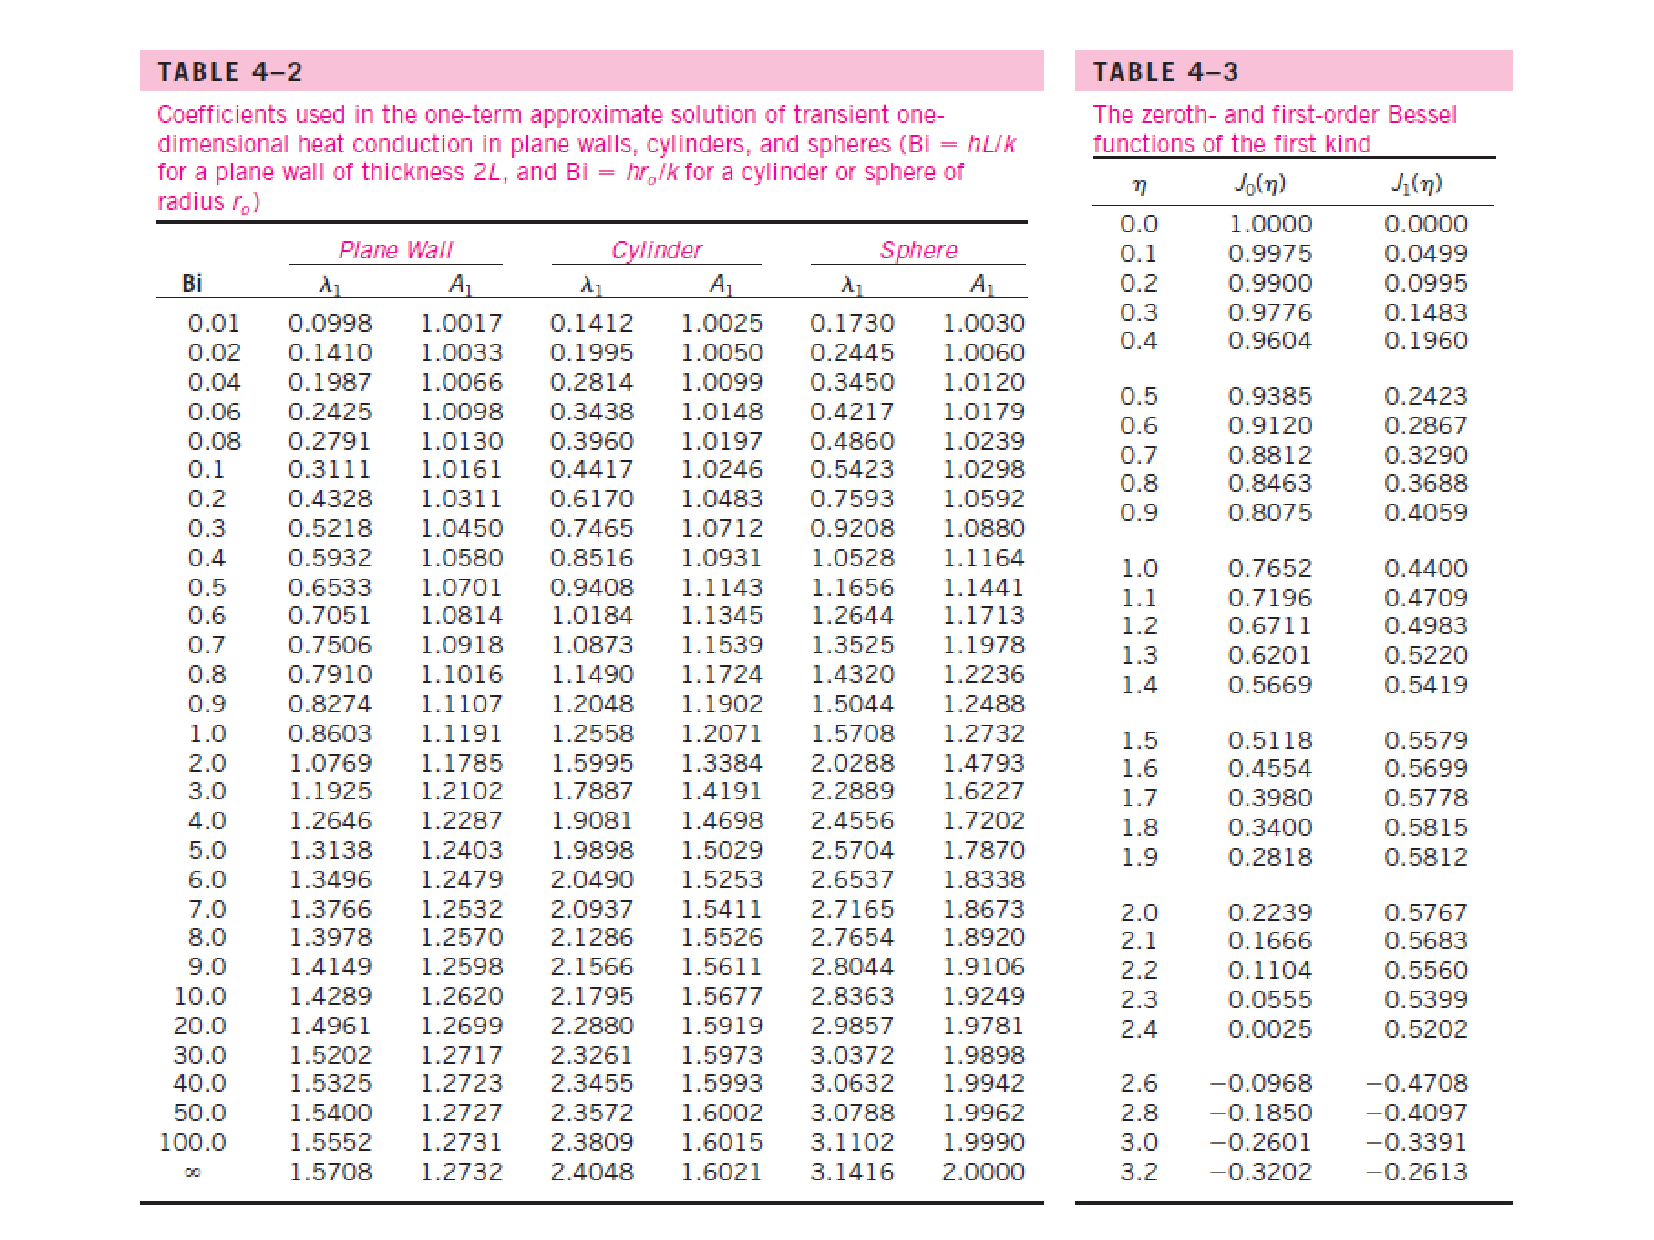
\includepdf[pages=-,fitpaper]{./Pics/BaselFunctionTable}
}


\end{document}
